\documentclass{article}
\usepackage{physics}
\usepackage{graphicx}
\usepackage{caption}
\usepackage{amsmath}
\usepackage{bm}
\usepackage{framed}
\usepackage{authblk}
\usepackage{empheq}
\usepackage{amsfonts}
\usepackage{esint}
\usepackage[makeroom]{cancel}
\usepackage{dsfont}
\usepackage{centernot}
\usepackage{mathtools}
\usepackage{subcaption}
\usepackage{bigints}
\usepackage{amsthm}
\theoremstyle{definition}
\newtheorem{lemma}{Lemma}
\newtheorem{defn}{Definition}[section]
\newtheorem{prop}{Proposition}[section]
\newtheorem{rmk}{Remark}[section]
\newtheorem{thm}{Theorem}[section]
\newtheorem{exmp}{Example}[section]
\newtheorem{prob}{Problem}[section]
\newtheorem{sln}{Solution}[section]
\newtheorem*{prob*}{Problem}
\newtheorem{exer}{Exercise}[section]
\newtheorem*{exer*}{Exercise}
\newtheorem*{sln*}{Solution}
\usepackage{empheq}
\usepackage{tensor}
\usepackage{xcolor}
%\definecolor{colby}{rgb}{0.0, 0.0, 0.5}
\definecolor{MIT}{RGB}{163, 31, 52}
\usepackage[pdftex]{hyperref}
%\hypersetup{colorlinks,urlcolor=colby}
\hypersetup{colorlinks,linkcolor={MIT},citecolor={MIT},urlcolor={MIT}}  
\usepackage[left=1in,right=1in,top=1in,bottom=1in]{geometry}
\usepackage{newpxtext,newpxmath}
\newcommand*\widefbox[1]{\fbox{\hspace{2em}#1\hspace{2em}}}
\newcommand{\p}{\partial}
\newcommand{\R}{\mathbb{R}}
\newcommand{\C}{\mathbb{C}}
\newcommand{\lag}{\mathcal{L}}
\newcommand{\nn}{\nonumber}
\newcommand{\ham}{\mathcal{H}}
\newcommand{\M}{\mathcal{M}}
\newcommand{\I}{\mathcal{I}}
\newcommand{\K}{\mathcal{K}}
\newcommand{\F}{\mathcal{F}}
\newcommand{\w}{\omega}
\newcommand{\lam}{\lambda}
\newcommand{\al}{\alpha}
\newcommand{\be}{\beta}
\newcommand{\x}{\xi}
\newcommand{\G}{\mathcal{G}}
\newcommand{\f}[2]{\frac{#1}{#2}}
\newcommand{\ift}{\infty}
\newcommand{\lp}{\left(}
\newcommand{\rp}{\right)}
\newcommand{\lb}{\left[}
\newcommand{\rb}{\right]}
\newcommand{\lc}{\left\{}
\newcommand{\rc}{\right\}}
\newcommand{\V}{\mathbf{V}}
\newcommand{\U}{\mathcal{U}}
\newcommand{\Id}{\mathcal{I}}
\newcommand{\D}{\mathcal{D}}
\newcommand{\Z}{\mathcal{Z}}

%\setcounter{chapter}{-1}

\usepackage{enumitem}
\usepackage{listings}
\captionsetup[lstlisting]{margin=0cm,format=hang,font=small,format=plain,labelfont={bf,up},textfont={it}}
\renewcommand*{\lstlistingname}{Code \textcolor{violet}{\textsl{Mathematica}}}
\definecolor{gris245}{RGB}{245,245,245}
\definecolor{olive}{RGB}{50,140,50}
\definecolor{brun}{RGB}{175,100,80}

%\hypersetup{colorlinks,urlcolor=colby}
\lstset{
	tabsize=4,
	frame=single,
	language=mathematica,
	basicstyle=\scriptsize\ttfamily,
	keywordstyle=\color{black},
	backgroundcolor=\color{gris245},
	commentstyle=\color{gray},
	showstringspaces=false,
	emph={
		r1,
		r2,
		epsilon,epsilon_,
		Newton,Newton_
	},emphstyle={\color{olive}},
	emph={[2]
		L,
		CouleurCourbe,
		PotentielEffectif,
		IdCourbe,
		Courbe
	},emphstyle={[2]\color{blue}},
	emph={[3]r,r_,n,n_},emphstyle={[3]\color{magenta}}
}

\begin{document}

\begin{center}
	\Large{Free-to-free thermal RF lineshape???}
\end{center}	

\begin{center}
	\today
\end{center}

\section{Context}

In our experiment we begin with a thermal mixture of $^{23}$ Na in the hyperfine state $\ket{F=1, m_F=1}$ and $^{40}$ K in the hyperfine state $\ket{F=9/2, m_F = -9/2}$ at around 100 G. A Blackman pulse of duration $\sim$100 ms with Rabi frequency $\sim$5 kHz is turned on. The frequency $\omega_\text{rf}$ of the rf field is tuned across the resonance for the $m_F = -9/2 \to m_F = -7/2$ hyperfine resonance in $^{40}$K. There are two relevant Na-K scattering lengths which we denote $a_{-9/2}$ and $a_{-7/2}$. At 100 G, we have $a_{-9/2} = -1698 a_0$ and $a_{-7/2} = 644 a_0$, which means there is a two-body bound state of NaK with  $\ket{^{23}\text{Na}, F=1, m_F=1}$ and $\ket{^{40} \text{K}, F=9/2, m_F = -9/2}$ and no bound state of NaK with $^{40}$ K in $m_F = -9/2$. It is thus possible to create these bound states (a.k.a. Feshbach molecules) using the rf field when $\omega_\text{rf}$ is an amount $E_b$ that is the molecule binding energy from the bare hyperfine resonance $\omega_\text{HF}$. The molecule association lineshape is known (see, for example, \cite{FB_rf_1}). \\

\noindent What we're after is the lineshape of the $^{40}$K $m_F = -9/2 \to m_F = -7/2$ transition in the presence of Na. In our experiment, we observed the lineshape to have a threshold behavior with a high-frequency tail. We know this has to do with the interaction with the Na bath, but have not found a satisfactory quantitative model for this rf response. The goal of this document is to put together what we know and what we need to know in order to find this lineshape. There are at least two ways to get the rf response for our system.

\section{Momentum conservation}

Consider a single $\ket{^{23}\text{Na}, F=1, m_F=1}$ atom interacting with a $\ket{^{40} \text{K}, F=9/2, m_F = -9/2}$ atom. Assume that the Na atom has momentum $\hbar k_\text{Na}$ and the K atom has momentum $\hbar k_{K}$. We assume that the rf field with detuning $\delta$ from the hyperfine resonance does not change the momentum of the two-body system. 


\section{Two-body scattering $T$-matrix}

We assume wo-body short-range contact interaction between the Na and K atoms. The bare interaction strength is given by 
\begin{align}
 \frac{1}{g} = \frac{\mu}{4\pi a_s} - \sum_k^\Lambda  \frac{1}{2\epsilon_\mathbf{k}} 
\end{align}
where $\mu$ is the Na-K reduced mass and $\epsilon_\mathbf{k}$ is the kinetic energy associated with the relative motion of the atoms. Just for clarity, we provide the reader with useful relations between the various momenta. These can be readily derived from the coordinate transformation, but it is nice to have them at our finger tips.
\begin{align}
P_\text{COM} = p_\text{Na} + p_\text{K}
\quad\quad\quad 
P_\text{rel} = \hbar k = \mu \left( \frac{p_\text{Na}}{m_\text{Na}} - \frac{p_\text{K}}{m_\text{K}}  \right)
\end{align}

\noindent The two-body scattering $T$-matrix is given in terms of the relative momentum $\hbar k$. As a reminder, the $T$-matrix is directly related to the scattering amplitude from the initial relative momentum  $\mathbf{k}$ to final relative momentum $\mathbf{k}'$ (see Eq. 7.2.19 of \cite{sakurai1995modern}):
\begin{align}
f(\mathbf{k}',\mathbf{k}) = -\frac{1}{4\pi} \frac{2\mu}{\hbar^2} (2\pi)^3 \bra{\mathbf{k}' } T \ket{\mathbf{k}}.
\end{align}

\noindent For the case of forward scattering, $\mathbf{k}' = \mathbf{k}$, and the amplitude is given by 
\begin{align}\label{eq:fwd-amplitude}
f(\mathbf{k}'=\mathbf{k},\mathbf{k}) = f(\theta = 0, k) =  -\frac{1}{4\pi} \frac{2\mu}{\hbar^2} (2\pi)^3 T(k). 
\end{align}

\noindent But we also know that for low-energy, $s$-wave scattering, the (forward) scattering amplitude is given by (see, for example, Eq. 7.6.16 of \cite{sakurai1995modern})
\begin{align}\label{eq:s-wave-amplitude}
f_{\ell = 0}(k) = \frac{1}{k\cot \delta_{\ell = 0} - ik}  = \frac{a}{1 - ika}.
\end{align}

\noindent We can now put together Eq. \eqref{eq:fwd-amplitude} and Eq. \eqref{eq:s-wave-amplitude} to get the commonly quoted expression for the $T$-matrix
\begin{align}\label{eq:T-matrix}
\boxed{T(\omega) =  \frac{4\pi}{2\mu} \frac{1}{a^{-1} - \sqrt{- 2\mu\omega}}}
\end{align}
where we have dropped certain factors of $\pi$ and $\hbar$ to adhere to conventions in the literature.\\

\noindent In the case of scattering between particles of equal mass, the reduced mass is $\mu = m^2/2m = m/2$. The two-body $T$-matrix is then:
\begin{align}
T(\omega) =  \frac{4\pi}{m} \frac{1}{a^{-1} - \sqrt{- m\omega}},
\end{align}
where we have made the replacement $ik \to \sqrt{-m\omega}$. This is the expression found in Meera's \cite{mulkerin2024rabi} and Leyronas's \cite{sun2015high}. Reinstating $\hbar$, we find that the $T$-matrix has a pole at $\omega = \hbar^2/2\mu a^2$ whenever $a > 0$. This is precisely the statement that the two-body problem admits a bound state when the interaction is repulsive. 



\section{Self-energy in the virial expansion for interacting equal mass fermions}

\subsection{Virial expansion of the Green's function}

Following \cite{sun2015high} and \cite{leyronas2011virial}, we begin with the propagator for a free fermion of mass $m_F$ in imaginary time:
\begin{align}\label{eq:free-fermion}
G^{(0)}(\mathbf{k}, \tau) = e^{-(\epsilon_\mathbf{k} - \mu)\tau} [ n_F(\epsilon_\mathbf{k} - \mu) - \Theta(\tau)]
\end{align}
where $\mu$ is the chemical potential, $\epsilon_\mathbf{k} = \hbar^2 k^2 / 2m_F$, $n_F(x) = 1/(e^{\beta x} + 1)$ is the Fermi-Dirac distribution, $\Theta(x)$ is the Heaviside step function, and $\tau$ is the imaginary time. The derivation for the free-fermion propagator can be found in many textbooks/lecture notes (see, for example, \href{https://webspace.science.uu.nl/~morai101/oldWebsite/public_html/SFT06four.pdf}{this page}), but we can reproduce it here:\\

\fbox{
\begin{minipage}{0.95\textwidth}
\noindent A free particle of mass $m$ has the Hamiltonian
\begin{align}
H = \sum_\mathbf{k} \epsilon_\mathbf{k} a^\dagger_\mathbf{k} a_\mathbf{k}
\end{align}
with $\epsilon_\mathbf{k} = \hbar^2 k^2 / 2m$, and $a^\dagger(t), a(t)$ the (time-dependent) creation and annihilation operators. The time independence comes in via $ a_\mathbf{k}(t) = e^{-i\epsilon_\mathbf{k} t / \hbar} a_\mathbf{k}(0) = e^{-i\epsilon_\mathbf{k} t / \hbar} a_\mathbf{k}$. The Green's function/propagator for the free particle is given by 
\begin{align}
G(\mathbf{k}, t) = -\langle \mathcal{T}[a_\mathbf{k}(t) a_\mathbf{k}^\dagger] \rangle
\end{align}
This is nothing but the amplitude of annihilating a particle of momentum $\hbar \mathbf{k}$ at $t'=0$ and creating a particle of momentum $\hbar \mathbf{k}$ at $t'=t$. Here, $\mathcal{T}[\cdot]$ denotes the time-ordering operator. For fermions, we have $\langle a_\mathbf{k}^\dagger a_\mathbf{k} \rangle = n_F(\mathbf{k})$ and $\mathcal{T}[\cdot] \to \mathcal{T}_F[\cdot]$ is the fermionic time-ordering operator. By applying the fermionic anti-commutation rule and plugging this into the definition for the Green's function, we find the result in Eq. \eqref{eq:free-fermion} after some small simplifications.
\end{minipage}
}\\\\


\noindent In the high-temperature limit, the Fermi-Dirac distribution can be expanded in powers of the fugacity $z = e^{\beta \mu} \ll 1$ as:
\begin{align}
n_F(\epsilon_\mathbf{k}, \mu) = \sum_{n\geq 1} (-1)^{n+1} z^n e^{-n\beta \epsilon_\mathbf{k}}.
\end{align}

\noindent The free fermion Green's function is then
\begin{align}
G^{(0)}(\mathbf{k}, \tau) = e^{\mu \tau} \left[ \sum_{n\geq 0} G^{(0,n)} (\mathbf{k}, \tau) z^n \right],
\end{align}
where 
\begin{align}
G^{(0,0)} (\mathbf{k}, \tau) &= -\Theta(\tau)e^{-\epsilon_\mathbf{k}\tau} \\
G^{(0,n)} (\mathbf{k}, \tau) &= (-1)^{n-1} e^{-\epsilon_\mathbf{k}\tau} e^{-n\beta \epsilon_\mathbf{k}}, \quad n\geq 1.
\end{align} 

\noindent We see that $G^{(0,0)}$ is retarded, but not $G^{(0,n)}$ for $n\geq 1$. In the language of Feynman diagrams, $G^{(0,0)}$ is a  line going from left to right in the direction of increasing time, while $G^{(0,n)}$ can go either way (see \cite{barth2014pairing} for an example of such a Feynman diagram). The leading order in $z$ is thus given by the diagram with the least number of advanced propagators. In this case it would be $G^{(0,1)}$.\\


\subsection{Self-energy}

\noindent The self-energy operator $\Sigma$ relates the free and dressed fermion Green's functions via 
\begin{align}
G = G^{(0)} + G^{(0)} \Sigma G \implies \Sigma = [G^{(0)}]^{-1} - [G]^{-1}.
\end{align}

\noindent We see that the contribution to the self-energy with the lowest order in $z$ is $G^{(0,1)}$. \\

\noindent For the case of interacting fermions of spins $\uparrow, \downarrow$ of equal mass, [Meera](https://arxiv.org/pdf/1309.0272.pdf) shows that the self-energy, to lowest order of $z$, has the form of an integral over some degrees of freedom of the $T$-matrix multiplied by $G^{(0,1)}$. The result is Eq. (5) of \cite{sun2015high}:
\begin{align}
\Sigma^{(1)}(\mathbf{k},\tau) = z \int \frac{d^3P}{(2\pi)^3} e^{\mu\tau} e^{-(\beta-\tau) \epsilon_\mathbf{P-k}} T(\mathbf{P},\tau).
\end{align}


\noindent This formula seems to be "out of the blue", but Meera \cite{ngampruetikorn2013pair} provides a Feynman diagram which better elucidates its origins. Basically, we want to think of the contribution to the self-energy of a particle with momentum $\hbar k$ to lowest order of $z$, due to another particle, is a product of the $T$-matrix and the advanced Green's function of that other particle (which has momentum $\mathbf{P} - \mathbf{k}$, where $\mathbf{P}$ is the total momentum), summed over all the possible values for $\mathbf{P}$ \cite{leyronas2011virial}. So, in the case of two interacting fermions of the equal mass, the self-energy has the form
\begin{align}
\Sigma^{(1)}_\uparrow(\mathbf{k}, \tau) \approx \int_P d\mathbf{P} \, G_\downarrow(\mathbf{P} - \mathbf{k},-\tau) T(\mathbf{P}, \tau).
\end{align}

\noindent How does the $T$-matrix $T(\mathbf{P},\tau)$ in the imaginary time domain relate to the $T$-matrix $T(\omega)$ in the frequency domain? The answer is that $T(\omega)$ is the Laplace transform of $T(\mathbf{P},\tau)$, or equivalently, $T(\mathbf{P}, \tau)$ is the inverse Laplace transform of $T(\omega)$. In the case of two interacting particles of equal mass, the total mass is $M = 2m$, so that 
\begin{align}
T(\mathbf{P},\tau) 
&=  \int_{C_\gamma} \frac{d\omega}{2\pi i} e^{-\tau \omega} T\left( \omega - \frac{P^2}{2M} \right) \\
&= e^{-\frac{\tau P^2}{4m}} \int_{C_\gamma} \frac{d\omega}{2\pi i} e^{-\tau \omega} T(\omega),
\end{align}
where we have made the change of variables $\omega \to \omega - \mathbf{P}^2/2M$. This is the "Galilean invariance" mentioned in \cite{sun2015high}, which gives $T(\mathbf{P},\tau) = e^{-P^2/4m} T(0,\tau)$. The contour $C_\gamma$ is called the Bromwich contour. We won't go into the details here, but since $T(\omega)$ is already known, we can compute this integral. The result is \cite{sun2015high}
\begin{align}
T(\mathbf{P}, \tau) = e^{-\frac{\tau P^2}{4m}} \left[ \Theta(a^{-1}) Z_m e^{E_b \tau} + \int_0^\infty e^{-\tau x} \rho(x)\,dx\right].
\end{align}

\noindent Here $Z_m = \pi / \mu^2 a = 4\pi / m^2 a$ is the molecular residue, and 
\begin{align}
\rho(x) 
= -\frac{1}{\pi} \,\text{Im}[T(x + i0^+)] 
= \frac{4}{\mu^{3/2}} \frac{\sqrt{x}}{x + E_b}
\end{align}
is the spectral density of the $T$-matrix. It is worthwhile to prove the second equality:\\

\fbox{
\begin{minipage}{0.95\textwidth}
Using our definition for the $T$-matrix, the derivation here will give a result that is different by a constant multiplicative factor compared to what is given by \cite{sun2015high}, but we will see why:
\begin{align}
-\frac{1}{\pi} \,\text{Im}[T(x + i0^+)] 
&= -\frac{1}{\pi} \lim_{\eta \to 0^+} \text{Im}[T(x+i\eta)] \\
&= 
-\frac{1}{\pi} \lim_{\eta \to 0^+}   
\frac{2\sqrt{2}\pi}{\mu} \sqrt[4]{\mu^2 \eta^2+\mu^2 x^2} \sin \left(\frac{1}{2} \arg (-\mu (x+i\eta))\right) \\
&\quad\times 
\left\{ 
\left[\frac{1}{a}-\sqrt{2} \sqrt[4]{\mu^2 \eta^2+\mu^2 x^2} \cos
   \left(\frac{1}{2} \arg (-\mu (x+i \eta))\right)\right]^2 \right. \\
   & \quad\quad\quad\left.+ 2 \sqrt{\mu^2 \eta^2+\mu^2 x^2} \sin^2\left(\frac{1}{2} \arg (-\mu (x+i \eta))\right)
\right\}^{-1}\\
&= 
\frac{1}{\pi}
\frac{2\sqrt{2}\pi}{\mu}
\frac{\sqrt[4]{\mu^2 x^2}}
{\frac{1}{a^2}+
2 \sqrt{\mu^2 x^2}} \\
&= 
\frac{1}{\pi} \frac{2\sqrt{2} \pi \sqrt{{x}}}{\sqrt{\mu}\left( \frac{1}{a^2} + 2\mu {x}\right)} \\
&= 
\frac{2\sqrt{2}}{\mu^{3/2}} \frac{\sqrt{{x}}}{{x} + \frac{1}{2\mu a^2}}\\
&= 
\frac{2\sqrt{2}}{\mu^{3/2}} \frac{\sqrt{{x}}}{{x} + E_b}.
\end{align}
The factor $2\sqrt{2}$ becomes $4$ when $\mu = m/2$, so we're in agreement with \cite{sun2015high}. In order to go from the first to the second line, we have used the function \texttt{ComplexExpand[]} in \texttt{Mathematica}.
\end{minipage}
}\\\\


\noindent Leyronas interprets the expression for $T(\mathbf{P}, \tau)$ as follows: the first term comes from the two-body bound state (which exists in the case where $a>0$), while the second term comes from the two-particle scattering states continuum of energy $x$. Putting this expression back into the expression for the self-energy, we find to first order in $z$ after Fourier-transforming (via Matsubara frequencies -- I don't really understand this) and analytically-continuing: 
\begin{align}
\Sigma^{(1)}(\mathbf{k}, \omega) \approx z F(\mathbf{k}, \omega + \mu + i0^+),
\end{align}
where
\begin{align}
F(\mathbf{k}, E) = \int \frac{d\mathbf{P}}{(2\pi)^3} e^{-\beta  \frac{(\mathbf{P}- \mathbf{k})^2}{2m}}
\left\{
\int_0^\infty \,\,dx \frac{\rho(x)}{E - \left[ \frac{P^2}{4m} + x - \frac{(\mathbf{P} - \mathbf{k})^2}{2m} \right]}
+
\Theta(a^{-1})\frac{Z_m}{E - \left[ \frac{\mathbf{P}^2}{4m} - E_b - \frac{(\mathbf{P} - \mathbf{k})^2}{2m}\right]}
\right\}.
\end{align}

\noindent The case of interacting fermions ($\uparrow, \downarrow$) of equal masses is then done, at least to first order in $z$. From the self-energy, we can then compute the retarded Green's function via the Dyson's equation. The spectral function is directly related to the imaginary part of the Green's function. Following \cite{haussmann2009spectral}, one can then extract the rf response from the spectral function depending on the initial and final states. 


\subsection{Spectral function}

The spectral function is computed from the identity
\begin{align}
A(\mathbf{k}, \omega) = -\f{1}{\pi}\text{Im}(G_R(\mathbf{k}, \omega)),
\end{align}
where the retarded Green's function $G_R(\mathbf{k}, \omega)$ is given by 
\begin{align}
G_R(\mathbf{k}, \omega) = \f{1}{\omega + \mu + i0^+ - \epsilon_\mathbf{k} - \Sigma_R(\mathbf{k}, \omega)}.
\end{align}
In order to proceed with this calculation, we have to know the real and imaginary parts of the retarded self-energy. Due to  Eq. \eqref{eq:BF-self-energy} and subsequently Eq. \eqref{eq:BF-F-function}, this comes down to finding the real and imaginary parts of the $T$-matrix for $\omega + i0^+$ in the frequency domain, which we fortuitously already found.\\

\noindent The resulting spectral function is given by 
\begin{align}
A(\mathbf{k}, \omega) 
&\propto
\frac
{-2 \text{ Im}[\Sigma^{(1)}(\mathbf{k}, \omega + \mu)]}
{
(\omega + \mu -\epsilon_\mathbf{k} - \text{Re}[\Sigma^{(1)}(\mathbf{k}, \omega + \mu)])^2 
+
\text{ Im}[\Sigma^{(1)}(\mathbf{k}, \omega + \mu)]^2
}
\end{align}

\noindent We now need to evaluate the function $F$:
\begin{align}
F(\mathbf{k}, E) 
&= \int \frac{d\mathbf{P}}{(2\pi)^3} e^{-\beta \frac{(\mathbf{P} - \mathbf{k})^2}{2m}} 
T\left( E - \frac{\mathbf{P}^2}{4m} + \frac{(\mathbf{P} - \mathbf{k})^2}{2m} \right),
\end{align}

\noindent The imaginary part of $F$ can be found by substituting in the expression for the imaginary part of the $T$-matrix. The real part of $F$ can be found by using the full expression of the $T$-matrix and taking the real part of the result of the integration. The integration that is to follow is done using in \texttt{Python}'s package \texttt{scipy.integrate.quad}. The trick to not get weird results is actually to let Python know that the integrand is complex and to avoid hitting the pole on the real axis by shifting the argument $E$ by a small imaginary part $E \to E + i\eta$. \\

\noindent In order to get some qualitative behavior of $F(\mathbf{k}, E)$ and eventually $A(\mathbf{k}, \omega)$, let us assume for simplicity that $\hbar = m = 1$. Moreover, assume that energies are in units of $1/\beta = k_B T = 1$ and that the scattering length is $a = 0.2$, so that the binding energy is $E_b = 1/(2 \times 0.2^2) = 12.5$. For the integral, we integrate over $P$ from 0 to a momentum cutoff of $100$.  \\

\noindent Python code: 
\begin{lstlisting}
(*Code for the integrands*)
from scipy.integrate import quad

def imaginary_integrand(P, En, a_scat):
    s = En + 0.1j + P**2
    Eb = 1/(2 * a_scat**2)
    return -4*np.pi*(P**2)*np.exp(-P**2) * np.sqrt(s)/ (s + Eb)

def real_integrand(P, En, a_scat):
    s = En + 0.1j + P**2
    return (P**2)*np.exp(-P**2) / (1/a_scat - np.sqrt(-s))
    
(*Code for calculating real and imaginary parts*)
points = 500
momentum_cutoff = 100
En = np.linspace(-25,25,points)
a_scat = 0.2
imaginary_results = []*points
real_results = []*points
for i in range(points):
    real_results.append(quad(real_integrand, 0, momentum_cutoff, args=(En[i], a_scat))[0])
    imaginary_results.append(quad(imaginary_integrand, 0, momentum_cutoff, args=(En[i], a_scat))[0])
    
(*Plot the spectral function*)
A =  -2* np.array(imaginary_results)/( (En + np.array(real_results))**2 + np.array(imaginary_results)**2)
plt.plot(En,A)
plt.ylim([0,0.05])
plt.grid()
plt.xlabel('rf frequency (arb)')
plt.ylabel('Spectral function')
plt.show()
\end{lstlisting}


\begin{figure}[!htb]
\begin{minipage}{.5\textwidth}
  \centering
  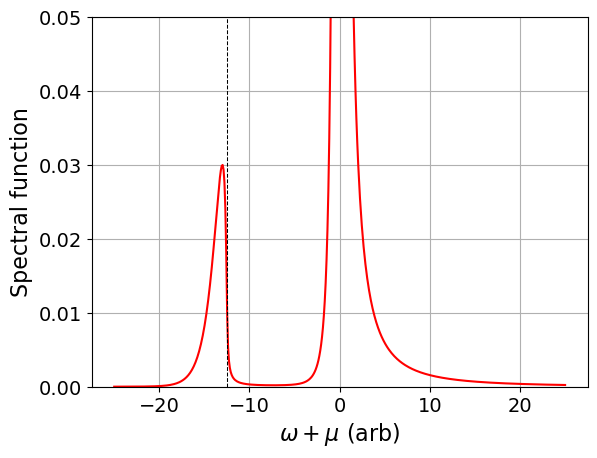
\includegraphics[width=.95\linewidth]{A_fermions_1}
\end{minipage}%
\begin{minipage}{.5\textwidth}
  \centering
  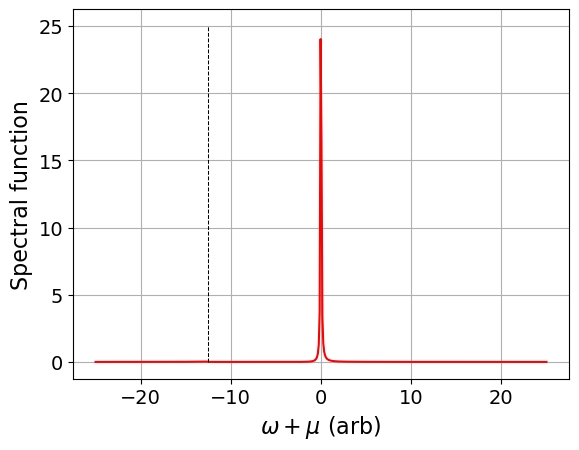
\includegraphics[width=.95\linewidth]{A_fermions_2}
\end{minipage}
\caption{Spectral function $A(0, \omega)$. The dashed black line on the left figure denotes frequency $\omega + \mu = -E_b$, marking the onset for the molecule association lineshape. The feature on the right of the molecular feature is the free-to-free lineshape. It is the noninteracting free-particle spectrum, modified by two-body contact interaction. The figure on the right shows the full spectrum. The single-particle peak has much larger spectral weight compared to the molecular peak.}
\label{fig:fermion-spectrum}
\end{figure}


\noindent Figure \ref{fig:fermion-spectrum} shows the result of the calculation for the case of $\mathbf{k} = 0$. This plot is similar to Figure 2a of \cite{sun2015high}.  and Figure 2 of \cite{nishida2013electron}. For more detailed studies of how $A(\mathbf{k}, \omega)$ as a function of $\mathbf{k}$ and the scattering length $a$, refer to \cite{sun2015high}, for example. We're more interested in applying the formalism developed here to tackle our problem of a fermion impurity interacting with a boson bath.



\section{Self-energy a fermion interacting with a boson of unequal mass}

We would like to treat a slightly different scenario, with two main differences: the interacting particles have different quantum statistics and unequal mass. The self-energy for the fermion is now different: it is now the convolution of the $T$-matrix with the boson Green's function \cite{kharga2017single}, \cite{manabe2019single}. The self-energy for the fermion looks like
\begin{align}
\Sigma_F\sim \sum T \times G_B,
\end{align}
where $T$ denotes the two-body $T$-matrix and $G_B$ is the bosonic Green's function. To make the formalism consistent with what was done in the previous section, we should also find a virial expansion for this and obtain the self-energy to lowest order of the fugacity $z$. 

\subsection{Virial expansion of the Green's function}
\noindent We now attempt to obtain the free boson Green's function in the virial expansion. First, we expand the Bose-Einstein distribution in powers of the fugacity $z_B = e^{\beta \mu_B}$:
\begin{align}
n_B(\mathbf{k},\mu) = \frac{1}{e^{\beta(\epsilon_\mathbf{k} - \mu_B)} - 1} = \sum_{n\geq 1} z^n e^{-n \beta \epsilon_\mathbf{k}}.
\end{align}

\noindent Next, we find the free boson Green's function from the steps outlined in the beginning of the previous section:
\begin{align}
G_B^{(0)}(\mathbf{k}, \tau) 
&=  -e^{-(\epsilon_\mathbf{k} - \mu_B)\tau} 
\left\{
    [1 + n_B(\epsilon_\mathbf{k} - \mu_B) ] \Theta(\tau) +  n_B(\epsilon_\mathbf{k} - \mu_B) \Theta(-\tau)
\right\} \\
&= -e^{-(\epsilon_\mathbf{k} - \mu_B) \tau} [n_B(\epsilon_\mathbf{k} - \mu_B)  + \Theta(\tau) ].
\end{align}

\noindent In powers of the fugacity $\mu_B$, we have
\begin{align}
G^{(0)}_B(\mathbf{k}, \tau) = e^{\mu_B \tau} \sum_{n\geq 0} G_B^{(0,n)} (\mathbf{k}, \tau) z^n
\end{align}
where
\begin{align}
G_B^{(0,0)} (\mathbf{k}, \tau) &= -\Theta(\tau)e^{-\epsilon_\mathbf{k}\tau} \\
G_B^{(0,n)} (\mathbf{k}, \tau) &= e^{-\epsilon_\mathbf{k}\tau} e^{-n\beta \epsilon_\mathbf{k}}, \quad n\geq 1.
\end{align} 


\subsection{Self-energy}

\noindent The two-body $T$-matrix describing scattering between a fermion of mass $m_F$ and a boson of mass $m_B$ was already found. It is Eq. \eqref{eq:T-matrix}. Following the formalism by \cite{sun2015high}, the fermion self-energy to is gotten (approximately) from multiplying the $T$-matrix with the free bosonic Green's function, then integrating over all total momentum $\mathbf{P}$:
\begin{align}
\Sigma_F(\mathbf{k}, \tau) 
&\approx z e^{\mu_B \tau}\int \frac{d\mathbf{P}}{(2\pi)^3} G_B^{(0,1)}(\mathbf{P} - \mathbf{k}, -\tau) \, T(\mathbf{P}, \tau) \\
&=  z e^{\mu_B \tau} \int \frac{d\mathbf{P}}{(2\pi)^3} e^{-(\beta - \tau)\epsilon^B_{\mathbf{P}-\mathbf{k}}} \, T(\mathbf{P}, \tau),
\end{align}

\noindent The Feynman diagram for the fermionic self-energy for the case of a fermion interacting with a boson can be found in \cite{kharga2017single} and \cite{manabe2019single}, for instance. Just to be explicit here: the momentum of the fermion is $\mathbf{k}$, and the momentum of the boson is $\mathbf{P} - \mathbf{k}$, with $\mathbf{P}$ being the total momentum. The expression for $T(\mathbf{P}, \tau)$ is found in the previous section:
\begin{align}
T(\mathbf{P}, \tau) = e^{-\frac{\tau P^2}{2M}} \left[ \Theta(a^{-1}) Z_m e^{E_b \tau} + \int_0^\infty e^{-\tau x} \rho(x)\,dx\right],
\end{align}
but now the total mass is $M = m_\text{Na} + m_\text{K}$ and the molecular residue $Z_m = \pi / \mu^2 a$ is in terms of the reduced mass $\mu$. The function $\rho(x)$ is also already found from the previous section:
\begin{align}
\rho(x) 
= -\frac{1}{\pi} \,\text{Im}[T(x + i0^+)] 
= \frac{2\sqrt{2}}{\mu^{3/2}} \frac{\sqrt{x}}{x + E_b}.
\end{align}

\noindent Converting $\Sigma_F(\mathbf{k}, \tau)$ into its frequency-domain counter part (\textcolor{purple}{via Fourier-transforming over the Matsubara frequencies???}) and analytically continuing, we find 
\begin{align}\label{eq:BF-self-energy}
\Sigma_F(\mathbf{k}, \omega) =  z \, F(\mathbf{k}, \omega + \mu_B + i0^+),
\end{align}
where
\begin{align}
F(\mathbf{k}, E) = \int \frac{d\mathbf{P}}{(2\pi)^3} e^{-\beta  \frac{(\mathbf{P}- \mathbf{k})^2}{2m_\text{Na}}}
\left\{
\int_0^\infty \,dx \frac{\rho(x)}{E - \left[ \frac{\mathbf{P}^2}{2M} + x - \frac{(\mathbf{P} - \mathbf{k})^2}{2m_\text{Na}} \right]}
+
\Theta(a^{-1})\frac{Z_m}{E - \left[ \frac{\mathbf{P}^2}{2M} - E_b - \frac{(\mathbf{P} - \mathbf{k})^2}{2m_\text{Na}}\right]}
\right\}.
\end{align}
\textcolor{purple}{I once again don't know how this Fourier transform is done exactly. I would expect a Lorentzian because the object being transformed is an exponential in the imaginary time variable, but apparently that's not the case?} In any case, Leyronas claims that this function $F(\mathbf{k}, E)$ can be further simplified by observing that the $T$-matrix can be put into the form
\begin{align}
T(\omega) = \Theta(a^{-1}) \frac{Z_m}{\omega + E_b} + \int_0^\infty \,dx \frac{\rho(x)}{\omega - x},
\end{align}
which we can verify directly by plugging it into Mathematica (or doing the integral by hand). From here, \cite{sun2015high} is able to simplify the expression for the function $F$ to:
\begin{align}\label{eq:BF-F-function}
F(\mathbf{k}, E) = \int \frac{d\mathbf{P}}{(2\pi)^3} e^{-\beta \frac{(\mathbf{P} - \mathbf{k})^2}{2m_\text{Na}}} T\left( E - \frac{\mathbf{P}^2}{2M} + \frac{(\mathbf{P} - \mathbf{k})^2}{2m_\text{Na}} \right).
\end{align}


\subsection{Spectral function}

The spectral function is computed from the identity
\begin{align}
A(\mathbf{k}, \omega) = -\f{1}{\pi}\text{Im}(G_R(\mathbf{k}, \omega)),
\end{align}
where the retarded Green's function $G_R(\mathbf{k}, \omega)$ is given by 
\begin{align}
G_R(\mathbf{k}, \omega) = \f{1}{\omega + \mu + i0^+ - \epsilon_\mathbf{k} - \Sigma_R(\mathbf{k}, \omega)}.
\end{align}
In order to proceed with this calculation, we have to know the real and imaginary parts of the retarded self-energy. Due to  Eq. \eqref{eq:BF-self-energy} and subsequently Eq. \eqref{eq:BF-F-function}, this comes down to finding the real and imaginary parts of the $T$-matrix for $\omega + i0^+$ in the frequency domain, which we fortuitously already found.\\

\noindent The resulting spectral function is given by 
\begin{align}
A(\mathbf{k}, \omega) 
&\propto
\frac
{-2 \text{ Im}[\Sigma^{(1)}(\mathbf{k}, \omega + \mu)]}
{
(\omega + \mu -\epsilon_\mathbf{k} - \text{Re}[\Sigma^{(1)}(\mathbf{k}, \omega + \mu)])^2 
+
\text{ Im}[\Sigma^{(1)}(\mathbf{k}, \omega + \mu)]^2
}
\end{align}

\noindent We now need to evaluate the function $F$:
\begin{align}
F(\mathbf{k}, E) 
&= \int \frac{d\mathbf{P}}{(2\pi)^3} e^{-\beta \frac{(\mathbf{P} - \mathbf{k})^2}{2m_\text{Na}}} 
T\left( E - \frac{\mathbf{P}^2}{2M} + \frac{(\mathbf{P} - \mathbf{k})^2}{2m_\text{na}} \right),
\end{align}

\noindent The imaginary part of $F$ can be found by substituting in the expression for the imaginary part of the $T$-matrix. The real part of $F$ can be found by using the full expression of the $T$-matrix and taking the real part of the result of the integration. The integration that is to follow is done using in \texttt{Python}'s package \texttt{scipy.integrate.quad}. The trick to not get weird results is actually to let Python know that the integrand is complex and to avoid hitting the pole on the real axis by shifting the argument $E$ by a small imaginary part $E \to E + i\eta$. \\

\noindent We now want to evaluate the spectral function using physical values for the variables. \textcolor{red}{In progress: see Python code. I think I managed to plug in some quantities to get some no-nonsense spectral function, but I need to check for dangling factors of $\pi$'s and $\sqrt{2}$ so I'm not 100\% confident in the result yet, but it seems promising. Check the Jupyter notebook for this.}


\section{$\mathcal{O}(z^2)$ contributions to $\Sigma(\mathbf{k},\omega)$ and effects on $A(\mathbf{k}, \omega)$}




\section{RF response}

In experiments, the RF field transfers atoms from an occupied spin state into an empty final state. From the previous sections, we have found the spectral functions for both. Let's assume that the rf field flips the spin $\uparrow$ to $\downarrow$. Within linear response, the rate of transitions out of the initial state induced by the rf field with frequency $\omega$ and wave vector $\mathbf{q}$ is given by the convolution 
\begin{align}
I(\mathbf{q}, \omega)
\propto 
\int \f{d^3 k}{(2\pi)^3} \int d\epsilon \, A_\downarrow(\mathbf{k} + \mathbf{q}, \epsilon + \hbar \omega) A_\uparrow(\mathbf{k}, \epsilon) e^{-\be \epsilon}.
\end{align}
Here, unwritten is a prefactor that depends on the coupling strength to the rf field. Since the momentum transfer due to the rf field is very small, we can simply set $\mathbf{q} = 0$. With this simplification, the rf spectrum is 
\begin{align}
I(\omega) 
\propto
\int \f{d^3k}{(2\pi)^3} 
\int d\epsilon \, A_\downarrow(\mathbf{k}, \epsilon + \hbar \omega) A_\uparrow(\mathbf{k}, \epsilon)
\end{align}
If the final state is non-interacting, its spectral function is a delta-function:
\begin{align}
A_{\downarrow, \text{non-interacting}} (\mathbf{k},\epsilon) 
\propto
\delta(\epsilon - \epsilon_\mathbf{k}).
\end{align}
This gives the rf response function for this case:
\begin{align}
I_{\downarrow \text{ non-interacting}}(\omega) \propto 
\hbar \int \f{d^3k}{(2\pi)^3}  A_\uparrow(\mathbf{k}, \epsilon_\mathbf{k} - \hbar \omega).
\end{align}


\bibliography{free-to-free-lineshape} 
\bibliographystyle{unsrt}	

\end{document}